\documentclass[paper.tex]{subfiles}

\usepackage{tikz}
\usetikzlibrary{arrows.meta}

\usepackage{amsmath}
\usepackage{graphicx}
\usepackage{tabularx}
\usepackage{multicol}
\usepackage{algpseudocode}
\usepackage{algorithm}

% Add vertical spacing to tables
\renewcommand{\arraystretch}{1.4}

% Begin Document
\begin{document}

\begin{figure}[h]
\begin{center}
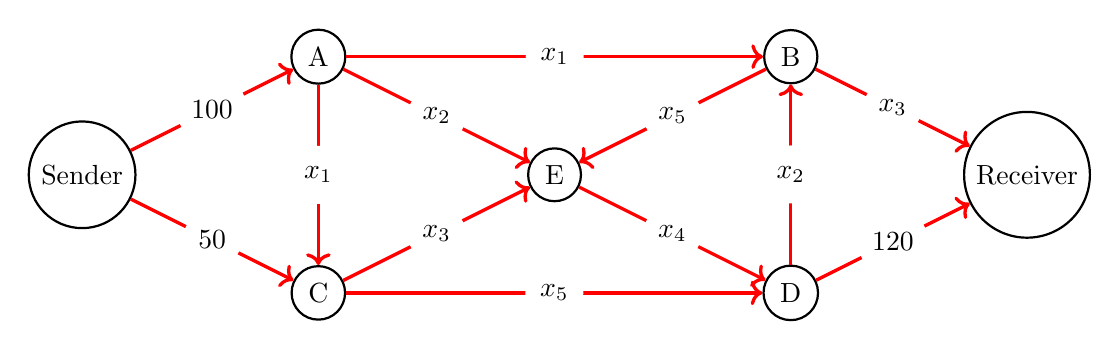
\begin{tikzpicture}

    \begin{scope}[every node/.style={circle,thick,draw}]
        \node (1) at (0,3) {A};
        \node (2) at (6,3) {B};
        \node (3) at (0,0) {C};
        \node (4) at (6,0) {D};
        \node (5) at (3,1.5) {E};
        \node (6) at (-3,1.5) {Sender};
        \node (7) at (9, 1.5) {Receiver};
    \end{scope}

    \begin{scope}[every node/.style={fill=white,circle}, every edge/.style={draw=red,very thick}]
        \path [->] (6) edge node {$100$} (1);
        \path [->] (6) edge node {$50$}  (3);
        \path [->] (1) edge node {$x_1$} (3);
        \path [->] (1) edge node {$x_1$} (2);
        \path [->] (1) edge node {$x_2$} (5);
        \path [->] (3) edge node {$x_3$} (5);
        \path [->] (3) edge node {$x_5$} (4);
        \path [->] (2) edge node {$x_5$} (5);
        \path [->] (5) edge node {$x_4$} (4);
        \path [->] (4) edge node {$x_2$} (2);
        \path [->] (2) edge node {$x_3$} (7);
        \path [->] (4) edge node {$120$} (7);
    \end{scope}

\end{tikzpicture}

\caption{The Network Graph}
\end{center}
\end{figure}

\end{document}